\documentclass[12pt,a4paper]{abntex2}
\usepackage[utf8]{inputenc}
\usepackage{amsmath}
\usepackage{esint}
\usepackage{amsfonts}
\usepackage{amssymb}
\usepackage{graphicx}
\usepackage{subfig}
\graphicspath{{fig/}}
\providecommand{\norm}[1]{\lVert#1\rVert}
\usepackage{empheq}
\usepackage{lscape}


\begin{document}

\tableofcontents

\chapter{Introdu\c{c}\~ao}
Como podemos constatar em \cite{eringen_1963}, existe uma similaridade matem\'tica entre a propaga\c{c}\~ao de ondas eletromagn\'eticas e el\'asticas em camadas que comp\~oem a subsuperf\'icie terrestre, que faz com que todas essas ondas tridimensionais possam ser representadas por equa\c{c}\~oes que possuem as mesmas propriedades. Verificamos tamb\'em que \'e poss\'ivel realizar o acoplamento dessas ondas, dentro de uma teoria conhecida como \textit{magnetoelasticidade}. Assim, segundo \cite{Ursin-1983}, podemos aplicar a mesma abordagem para tratamento tanto de ondas ac\'usticas como de ondas eletromagn\'eticas, e esse trabalho visa fazer o levantamento te\'orico de tal aplica\c{c}\~ao. A abordagem consiste basicamente em usar as tranformadas de Fourier, Laplace e Bessel no sistema de equa\c{c}\~oes diferenciais parciais que descrevem o acoplamento magnetoel\'astico, escrevendo-o em fun\c{c}\~ao da frequ\^encia temporal e numa forma matricial. Atrav\'es de transforma\c{c}\~ao das coordenadas laterais, o sistema \'e deixado em fun\c{c}\~ao apenas da profundidade e o sistema inical de EDP's \'e transformado em dois sistemas de equa\c{c}\~oes diferenciais ordin\'arias onde cada grandeza pode ser claculada separadamente. Tal procedimento \'e denominado \textit{m\'etodo matricial}.

Alguns pesquisadores j\'a utilizaram o m\'etodo matricial em sistema acoplados. \cite{White_Zhou_2006} utilizaram em m\'etodos de \textit{Eletros\'ismica} que estuda a convers\~ao de ondas eletromagn\'eticas em ondas s\'ismicas na subsuperf\'icie terrestre na prospec\c{c}\~ao de hidrocarbonetos. A convers\~ao entre as ondas ocorre em meios porosos onde uma onda eletromagn\'etica pode excitar uma onda s\'ismica de mesma frequ\^encia e vice-versa, atrav\'es do movimento dos fluidos contidos nos poros. A altera\c{c}\~ao que uma onda eletromagn\'etica promove numa onda s\'ismica de mesma frequ\^encia pode ser registrada na superf\'icie terrestre trazendo informa\c{c}\~oes sobre as propriedades el\'etricas da subsuperf\'icie. 

\cite{Azeredo_2013} aplica o m\'etodo matricial para resolver de forma anal\'itico-num\'erica equa\c{c}\~oes de poroelasticidade que descrevem a propaga\c{c}\~ao de ondas em meio plano estratificado formado por camadas homog\^eneas e isotr\'opicas. O m\'etodo fornece f\'ormulas expl\'icitas para a constru\c{c}\~ao de algoritmo computacional  para obter a solu\c{c}\~ao do problema.
\chapter{Vetor de Onda e Transformada de Fourier}
Segundo Farlow, a EDP de uma onda 
\begin{equation}\label{eq.edp_geral}
\frac{\partial^2\mathbf{f}(\mathbf{x},t)}{\partial\,t^2}=\norm{\mathbf{v}}^2\nabla^2\mathbf{f}(\mathbf{x},t)
\end{equation}
possui a solu\c{c}\~ao de D'Alembert
\begin{equation}
\mathbf{f}(\mathbf{x},t)=\mathbf{g}_1(\mathbf{x}-\mathbf{v}\,t)+\mathbf{g}_2(\mathbf{x}+\mathbf{v}\,t),
\end{equation}
onde $\mathbf{x}=(x,y,z)^\top$ representa o espa\c{c}o $\mathbb{R}^3$, $\mathbf{v}$ \'e a \textit{velocidade} de propaga\c{c}\~ao da onda, $(\mathbf{x}\pm\mathbf{v}\,t)$ \'e a \textit{fase} da onda, $\mathbf{g}_1$ \'e a propaga\c{c}\~ao da onda no semiespa\c{c}o positivo de $x$ e $\mathbf{g}_2$ \'e a propaga\c{c}\~ao da onda no semiespa\c{c}o negativo de $x$.

De acordo com FULANO, ondas tridimensionais se propagam em formato esferoidal mas localmente podem ser tratadas como ondas planas, DEFINIR ONDAS PLANAS principalmente para raios distantes da fonte, e assim a solu\c{c}\~ao de uma onda pode ser dada pela superposi\c{c}\~ao dessas ondas planas.

No $\mathbb{R}^3$ o \textit{vetor de onda} $\mathbf{k}=(k_x,k_y,k_z)$ \'e aquele que aponta na dire\c{c}\~ao de propaga\c{c}\~ao da onda e sua magnitude, denominda \textit{n\'umero de onda}, \'e definida como 
\begin{equation}
\norm{\mathbf{k}}=k=\frac{\omega}{\norm{\mathbf{v}}},
\end{equation}
onde $\omega$ \'e a frequ\^encia temporal. Desta forma, a fase da onda pode ser escrita em termos do vetor de onda e da frequ\^encia como $(\mathbf{k}\cdot\mathbf{x}-\omega\,t)$, e a solu\c{c}\~ao da equa\c{c}\~ao \ref{eq.edp_geral} pode ser reescrita como uma superposi\c{c}\~ao de ondas planas
\begin{equation}
\mathbf{f}(\mathbf{x},t)=\mathbf{A}\,\sum_{\mathbf{k},\omega}{e^{i\,(\mathbf{k}\cdot\mathbf{x}-\omega\,t)}},
\end{equation}
onde $\mathbf{A}$ \'e a \textit{amplitude} da onda.

Segundo \cite{White_Zhou_2006}, para o caso $\mathbb{R}^2$ o \textit{vetor de onda horizontal} \'e definido como $\mathbf{k}=(k_x,k_y)^\top$, o \textit{n\'umero de onda horizontal} e a \textit{vagarosidade horizontal} s\~ao, respectivamente,
\begin{equation}
k=\sqrt{k_x^2+k_y^2}\qquad\text{e}\qquad\gamma=\frac{k}{\omega}.
\end{equation}
A vagarosidade vertical \'e definida como
\begin{equation}
\eta=\frac{1}{v_z},
\end{equation}
onde $v_z$ \'e a componente vertical da velocidade. Denotando o \textit{n\'umero de onda vertical} por $k_z$, temos que a \textit{vagarosidade vertical} pode ser escrita como
\begin{equation}
\eta=\frac{k_z}{\omega}.
\end{equation}
Combinando as vagarosidades horizontal e vertical, temos
\begin{equation}
\gamma^2+\eta^2=\frac{1}{\norm{\mathbf{v}}^2}\qquad\text{ou}\qquad\eta=\sqrt{\frac{1}{\norm{\mathbf{v}}^2}-\gamma^2}.
\end{equation}
Podemos definir as transformadas de Fourier direta e inversa entre o espa\c{c}o bidimensional e o vetor de onda horizontal, como
\begin{align*}
\mathbf{\widehat{f}}(k_1,k_2,z) &= \iint_{\mathbb{R}^2}\mathbf{f}(x,y,z)\,e^{-i(k_1x+k_2y)}dx\,dy\\\\
\mathbf{f}(x,y,z) &= \left(\frac{1}{2\,\pi}\right)^2\iint_{\mathbb{R}^2}\mathbf{\widehat{f}}(k_1,k_2,z)\,e^{i(k_1x+k_2y)}dk_1dk_2.
\end{align*}
O s\'imbolo $\,\widehat{.}\,$ denota a fun\c{c}\~ao no espa\c{c}o da transformada lateral de Fourier.

\chapter{Escrevendo as EDP's como um Sistema de EDO's}
Neste capitulo vamos aplicar algumas tecnicas como rotacao do sistema de coordenadas e Transformadas Laterais de Fourier em EDP's para que as mesmas possam ser escritas como um sistema de EDO's.

\section{Sistema de EDP's do Efeito Magnetoel\'astico}

Segundo \cite{eringen_1963}, o acoplamento entre ondas eletromagn\'eticas e el\'asticas se propagando no subsolo caracteriza o efeito magnetoel\'astico, e esse acoplamento pode ser modelado matematicamente atrav\'es de um sistema de equa\c{c}\~oes diferencias parciais. Conforme minha monografia, podemos aplicar uma s\'erie de hip\'oteses que visam simplificar e linearizar essas EDP's de forma que as mesmas possam receber um tratamento matem\'atico adequado no sentido de se obter numericamente os valores dos campos eletromagn\'eticos e el\'asticos envolvidos no sistema. Desta forma, vamos utilizar o m\'etodo matricial encontrado em \cite{Ursin-1983} na solu\c{c}\~ao do seguinte sistema de EDP's da magnetoelasticidade
\begin{align}\label{eq.mag_ela_1}
\nabla\times\mathbf{{E}}&=i\,\omega\,\mu_0\mathbf{{H}}\\\nonumber\\\label{eq.mag_ela_2}
\nabla\times\mathbf{{H}}&=(\sigma-i\,\epsilon\,\omega)\,\mathbf{{E}}+\mathbf{{v}}\times\sigma\mu_0\mathbf{H}^0\\\nonumber\\\label{eq.mag_ela_3}
-i\,\omega\rho\,\mathbf{{v}}&=\nabla\cdot{\tau} + \mathbf{{F}}\\\nonumber\\\label{eq.mag_ela_4}
{\tau}&=\lambda\,\nabla\cdot\mathbf{{u}}\cdot\,I + G\,(\nabla\,\mathbf{{u}}+\nabla\mathbf{{u}}^\top)\\\nonumber\\\label{eq.mag_ela_5}
\nabla\cdot\mathbf{{H}}&=0.
\end{align}
Estas equa\c{c}\~oes est\~ao no dom\'inio da frequ\^encia $\omega$, a depend\^encia do tempo \'e dada por $\exp{-i\,\omega\,t}$ e 
\begin{itemize}
\item $\mathbf{{E}}$ \'e o campo el\'etrico,
\item $\mathbf{{B}}$ \'e o campo magn\'etico,
\item $\mathbf{{D}}$ \'e o campo de densidade de fluxo el\'etrico,
\item $\mathbf{{H}}$ \'e o campo magn\'etico auxiliar,
\item $\tau$ \'e o tensor de tens\~oes,
\item $\mathbf{{u}}$ \'e o deslocamento do meio,
\item $\mathbf{{v}}$ \'e a velocidade de deslocamento do meio,
\item $\mathbf{{F}}$ \'e uma for\c{c}a aplicada ao meio,
\item $\mathbf{H}^0$ \'e campo geomagn\'etico,
\item $i$ \'e um n\'umero complexo,
\item $\omega$ \'e a frequ\^encia temporal,
\item $\mu_0$ \'e a permeabilidade magn\'etica no v\'acuo,
\item $\sigma$ \'e a condutividade do meio,
\item $\epsilon$ \'e a permissividade el\'etrica do meio,
\item $\rho$ \'e a densidade do meio,
\item $\lambda$ e $G$ s\~ao par\^ametros de Lam\`e.
\end{itemize}
Vamos definir $\sigma^*=(\sigma-i\,\epsilon\,\omega)$. No subsolo, por conta do regime quasi-estacion\'ario, $(\sigma>>\epsilon\,\omega)$  e  temos $\sigma^*=\sigma$. No ar, a condutividade \'e zero e a permeabilidade el\'etrica \'e pr\'oxima a do v\'acuo $\epsilon_0$, assim temos $\sigma^*=-i\,\epsilon_0\omega$.

No formato matricial, a equacao \ref{eq.mag_ela_1} pode ser escrita como
\begin{equation*}
\begin{pmatrix}
\frac{\partial\,E_3}{\partial\,y}-\frac{\partial\,E_2}{\partial\,z}\\
\frac{\partial\,E_1}{\partial\,z}-\frac{\partial\,E_3}{\partial\,x}\\
\frac{\partial\,E_2}{\partial\,x}-\frac{\partial\,E_1}{\partial\,y}
\end{pmatrix}
=
i\,\omega\,\mu_0\,
\begin{pmatrix}
H_1\\
H_2\\
H_3
\end{pmatrix}.
\end{equation*}
Aplicando as transformadas laterais de Fourier, dada em \ref{eq.trans_fourier_1}, temos
\begin{empheq}[left=\empheqlbrace]{align*}
-i\,k_y\widehat{E}_3-\frac{\partial\,\widehat{E}_2}{\partial\,z}&=i\,\omega\,\mu_0\widehat{H}_1\\
\frac{\partial\,\widehat{E}_1}{\partial\,z}+i\,k_x\widehat{E}_3&=i\,\omega\,\mu_0\widehat{H}_2\\
-i\,k_x\widehat{E}_2+i\,k_y\widehat{E}_1&=i\,\omega\,\mu_0\widehat{H}_3.
\end{empheq} 
Rotacionando o sistema de forma que a primeira coordenada esteja orientada no sentido do vetor de onda horizontal, usando o operador dado pela equacao \ref{eq.operador_rotacao}, e fazendo as simplificacoes, temos
\begin{empheq}[left=\empheqlbrace]{align*}
\frac{\partial\,\tilde{E}_2}{\partial\,z}&=-i\,\omega\,\mu_0\tilde{H}_1\\
\frac{\partial\,\tilde{E}_1}{\partial\,z}&=i\,\omega\,\mu_0\tilde{H}_2-i\,k\tilde{E}_3\\
\tilde{E}_2&=-\frac{\omega\,\mu_0}{k}\tilde{H}_3.
\end{empheq}

Observando que $\mathbf{v}=-i\,\omega\mathbf{u}$ depois de aplicada a transformada de Fourier no tempo, a equacao \ref{eq.mag_ela_2} pode ser escrita como
\begin{equation*}
\begin{pmatrix}
\frac{\partial\,H_3}{\partial\,y}-\frac{\partial\,H_2}{\partial\,z}\\
\frac{\partial\,H_1}{\partial\,z}-\frac{\partial\,H_3}{\partial\,x}\\
\frac{\partial\,H_2}{\partial\,x}-\frac{\partial\,H_1}{\partial\,y}
\end{pmatrix}
=
(\sigma-i\,\epsilon\,\omega)\,
\begin{pmatrix}
E_1\\
E_2\\
E_3
\end{pmatrix}
-i\,\omega\,
\begin{pmatrix}
u_2H_3^0-u_3H_2^0\\
u_3H_1^0-u_1H_3^0\\
u_1H_2^0-u_2H_1^0
\end{pmatrix}.
\end{equation*}
Aplicando as transformadas laterais de Fourier conforme a equacao \ref{eq.trans_fourier_1}, temos
\begin{empheq}[left=\empheqlbrace]{align*}
-i\,k_y\widehat{H}_3-\frac{\partial\,\widehat{H}_2}{\partial\,z}&=(\sigma-i\,\epsilon\,\omega)\,\widehat{E}_1-i\,\omega(u_2H_3^0-u_3H_2^0)\\
\frac{\partial\,\widehat{H}_1}{\partial\,z}+i\,k_x\widehat{H}_3&=(\sigma-i\,\epsilon\,\omega)\,\widehat{E}_2-i\,\omega(u_3H_1^0-u_1H_3)\\
-i\,k_x\widehat{H}_2+i\,k_y\widehat{H}_1&=(\sigma-i\,\epsilon\,\omega)\,\widehat{E}_3-i\,\omega(u_1H_2^0-u_2H_1^0).
\end{empheq}
Rotacionando o sistema usando o operador dado pela equacao \ref{eq.operador_rotacao}, e fazendo as simplificacoes, temos
\begin{empheq}[left=\empheqlbrace]{align*}
\frac{\partial\,\tilde{H}_2}{\partial\,z}&=-(\sigma-i\,\epsilon\,\omega)\,\tilde{E}_1+i\,\omega\,\tilde{H}_3^0\tilde{u}_2-i\,\omega\,\tilde{H}_2^0\tilde{u}_3\\
\frac{\partial\,\tilde{H}_1}{\partial\,z}&=(\sigma-i\,\epsilon\,\omega)\,\tilde{E}_2-i\,\omega\,k\,\tilde{H}_3-i\,\omega\,\tilde{H}_1^0\tilde{u}_3+i\,\omega\,\tilde{H}_3^0\tilde{u}_1\\
\tilde{H}_2&=-\frac{(\sigma-i\,\epsilon\,\omega)}{i\,k}\tilde{E}_3+\frac{\omega}{k}  \tilde{H}_2^0\tilde{u}_1-\frac{\omega}{k}\tilde{H}_1^0\tilde{u}_2.
\end{empheq}

A equacao \ref{eq.mag_ela_3} pode ser reescrita como

\begin{empheq}[left=\empheqlbrace]{align*}
-\omega^2\rho\,u_1&=\frac{\partial \tau_{11}}{\partial\,x}+\frac{\partial \tau_{12}}{\partial\,y}+\frac{\partial \tau_{13}}{\partial\,z}+F_1\\
-\omega^2\rho\,u_2&=\frac{\partial \tau_{21}}{\partial\,x}+\frac{\partial \tau_{22}}{\partial\,y}+\frac{\partial \tau_{23}}{\partial\,z}+F_2\\
-\omega^2\rho\,u_3&=\frac{\partial \tau_{31}}{\partial\,x}+\frac{\partial \tau_{32}}{\partial\,y}+\frac{\partial \tau_{33}}{\partial\,z}+F_3
\end{empheq}
Aplicando as transformadas laterais de Fourier, temos
\begin{empheq}[left=\empheqlbrace]{align*}
-\omega^2\rho\,\widehat{u}_1&=-i\,k_x\widehat{\tau}_{11}-i\,k_y\widehat{\tau}_{12}+\frac{\partial\widehat{\tau}_{13}}{\partial\,z}+\widehat{F}_1\\
-\omega^2\rho\,\widehat{u}_2&=-i\,k_x\widehat{\tau}_{21}-i\,k_y\widehat{\tau}_{22}+\frac{\partial\widehat{\tau}_{23}}{\partial\,z}+\widehat{F}_2\\
-\omega^2\rho\,\widehat{u}_3&=-i\,k_x\widehat{\tau}_{31}-i\,k_y\widehat{\tau}_{32}+\frac{\partial\widehat{\tau}_{33}}{\partial\,z}+\widehat{F}_3.
\end{empheq}
Aplicando a rotacao e simplificando as equacoes, temos
\begin{empheq}[left=\empheqlbrace]{align*}
-\omega^2\rho\,\tilde{u}_1&=-i\,k\tilde{\tau}_{11}+\frac{\partial\tilde{\tau}_{13}}{\partial\,z}+\tilde{F}_1\\
-\omega^2\rho\,\tilde{u}_2&=-i\,k\tilde{\tau}_{12}+\frac{\partial\tilde{\tau}_{23}}{\partial\,z}+\tilde{F}_2\\
-\omega^2\rho\,\tilde{u}_3&=-i\,k\tilde{\tau}_{13}+\frac{\partial\tilde{\tau}_{33}}{\partial\,z}+\tilde{F}_3.
\end{empheq}


\chapter{M\'etodo Matricial de Ursin para Solu\c{c}\~ao de EDP's}
Este cap\'itulo trata da utiliza\c{c}\~ao de um m\'etodo matricial para estudar a propaga\c{c}\~ao de ondas em subsuperf\'icie terrestre, conforme estruturado em \cite{Ursin-1983}. O m\'etodo utiliza um conjunto de transformadas para escrever um sistema de EDP's em dois sistemas de EDO's em forma matricial, de modo que se possa separar o campo de ondas em ascendentes e descendentes atrav\'es de uma decomposi\c{c}\~ao em autovetores. \'E poss\'ivel computar a matriz de propaga\c{c}\~ao das ondas e as matrizes de transmiss\~ao e reflex\~ao de ondas nas fronteiras entre camadas atrav\'es de propriedades de simetrias.

\section{Escrevendo as Equa\c{c}\~oes na Forma Matricial}

Sendo $\mathbf{x}=(x,y,z)^{\top}$ o espa\c{c}o $\mathbb{R}^3$ e aplicando as tranformadas de Fourier direta e inversa na forma
\begin{align*}
F(\omega,k_1,k_2,z) &= \iiint_{-\infty}^{\infty}f(t,x,y,z)\,e^{i\omega t-ik_1x-ik_2y}dt\,dxdy\\\\
f(t,x,y,z) &= \left(\frac{1}{2\,\pi}\right)^3\,\iiint_{-\infty}^{\infty}F(\omega,k_1,k_2,z)\,e^{-i\omega t+ik_1x+ik_2y}d\omega\,dk_1dk_2\,,
\end{align*}
podemos escrever um conjunto de EDP's que descevem a propaga\c{c}\~ao de ondas sismomagn\'eticas em camadas horizontais da subsuperf\'icie terrestre somente em fun\c{c}\~ao da profundidade $z$. 

A t\'itulo de exemplo, tanto as EDP's de Maxwell para o eletromagnetismo
\begin{align}\label{eq.faraday_ampere}\nonumber
\nabla\times\mathbf{E}&=-\frac{\partial}{\partial t}\mathbf{B}\\\\\nonumber
\nabla\times\mathbf{H}&=\sigma\mathbf{E}+\frac{\partial}{\partial t}\mathbf{D}+\mathbf{G}\,,
\end{align}
como as EDP's el\'asticas
\begin{align}\label{eq.cauchy_hooke}\nonumber
\rho\frac{\partial^2 \mathbf{U}}{\partial t^2}&=\nabla\cdot\tau+\mathbf{F}\\\\\nonumber
\tau&=\lambda\nabla\cdot \mathbf{U}\cdot I + \mu(\nabla \mathbf{U}+\nabla \mathbf{U}^*)\,,
\end{align}
podem ser escritas no formato matricial apresentado por Ursin. Cada um desses sistemas, isoladamente, pode ser escrito no formato 
\begin{align}\label{eq.matricial}
\frac{\partial\,\mathbf{B}}{\partial\,z} &= \pm\,i\,\omega\,A\,\mathbf{B} = \pm\,i\,\omega\,
\begin{bmatrix}
0&A_1\\
A_2&0
\end{bmatrix}\,
\begin{bmatrix}
\mathbf{B_1}\\
\mathbf{B_2}	
\end{bmatrix}\,,
\end{align}
onde o vetor $\mathbf{B}$ representa uma onda qualquer e n\~ao o campo magn\'etico dado em \ref{eq.faraday_ampere}.

A equação \ref{eq.matricial} tem as seguintes caracter\'isticas:
\begin{itemize}
\item $A_{2\,n\times2\,n}$ \'e uma matriz que pode ser particionada em quatro submatrizes $n\times n$, com submatrizes de zeros na diagonal principal e submatrizes sim\'etricas $A_1$ e $A_2$ na diagonal secund\'aria. As componentes de $A_1$ e $A_2$ s\~ao fun\c{c}\~oes dos par\^ametros das EDP's \ref{eq.faraday_ampere} e \ref{eq.cauchy_hooke}, s\~ao fun\c{c}\~oes de $z$ e tamb\'em do vetor real de retardamento $\mathbf{p}=\frac{\mathbf{k}}{\omega}$. Para meios de baixa atenua\c{c}\~ao das ondas, as matrizes $A_1$ e $A_2$ s\~ao reais; 
\item O vetor de onda $\mathbf{B}$ tem dimens\~ao $2n\times1$ e \'e particionado em dois vetores $\mathbf{B}_1$ e $\mathbf{B}_2$ com dimens\~ao $n\times1$ . As componentes do vetor de onda s\~ao escolhidas de forma que $\mathbf{B}$ seja cont\'inuo atrav\'es das fronteiras entre duas camadas;
\item  Para ondas el\'asticas, metade das componentes de $\mathbf{B}$ s\~ao zeros na superf\'icie livre, ou seja, existe uma matriz de permuta\c{c}\~ao $T_{2n\times2n}$ onde $T^{-1}=T^\top$ e tal que
\begin{equation*}
\begin{bmatrix}
\mathbf{V}_1(\mathbf{0})\\
\mathbf{0}
\end{bmatrix}
=T\,\mathbf{B}\quad\text{quando}\quad z = 0\,;
\end{equation*}
\item As componentes do vetor de onda $\mathbf{B}$ s\~ao escolhidas de forma que o fluxo de energia na dire\c{c}\~ao $z$ seja dado por
\begin{equation*}
J=-\frac{1}{4}(\mathbf{B}_1^H\mathbf{B}_2+\mathbf{B}_2^H\mathbf{B}_1)=-\frac{1}{4}\mathbf{B}^H\,M\, \mathbf{B}\,,
\end{equation*}
onde $H$ denota complexo conjugado transposto,
\begin{equation*}
M=
\begin{bmatrix}
0_{n\times n}&I\\
I&0_{n\times n}
\end{bmatrix}
\end{equation*}
e $I$ \'e uma matriz identidade $n\times n$.
\end{itemize}

Os m\'etodos a seguir s\~ao aplicados em equa\c{c}\~oes escritas no formato matricial \ref{eq.matricial}, com ondas se propagando numa pilha de camadas n\~ao homog\^eneas e assumimos que os par\^ametros das equa\c{c}\~oes s\~ao fun\c{c}\~oes cont\'inuas no interior de cada camada que dependem apenas da profundidade $z$. O modelo inclui pilha de camadas homog\^eneas com par\^ametros constantes por camada e consideramos o eixo $z$ como sendo positivo no sentido descendente.   

\section{Decomposi\c{c}\~ao em Ondas Ascendentes e Descentes}

Para realizar a decomposi\c{c}\~ao do vetor $\mathbf{B}$ em ondas ascendentes e descendentes aplicamos uma diagonaliza\c{c}\~ao em autovalores na matriz $A$ na forma
\begin{equation}\label{eq.diagonalizacao}
A=L\,\Lambda_1L^{-1}\,,
\end{equation}
onde $\Lambda_1$ \'e a matriz diagonal dos autovalores $\lambda_i$ para $i=1,2,...,n$, e $L$ \'e a matriz dos autovetores correspondentes,
\begin{equation*}
\Lambda_1=
\begin{bmatrix}
\Lambda&0\\
0&-\Lambda
\end{bmatrix}\,.
\end{equation*} 
A defini\c{c}\~ao de autovalores e autovetores \'e dada por
\begin{equation}\label{eq.sist_autovalores}
\begin{bmatrix}
0&A_1\\
A_2&0
\end{bmatrix}
\begin{bmatrix}
\mathbf{L_1}\\
\mathbf{L_2}
\end{bmatrix}
=
\lambda\,
\begin{bmatrix}
\mathbf{L_1}\\
\mathbf{L_2}
\end{bmatrix}
\end{equation}
e aplicando o procedimento
\begin{equation*}
\begin{bmatrix}
0&A_1\\
A_2&0
\end{bmatrix}
\begin{bmatrix}
0&A_1\\
A_2&0
\end{bmatrix}
\begin{bmatrix}
\mathbf{L_1}\\
\mathbf{L_2}
\end{bmatrix}
=
\lambda\,\lambda\,
\begin{bmatrix}
\mathbf{L_1}\\
\mathbf{L_2}
\end{bmatrix}\,,
\end{equation*}
podemos separar o sitema \ref{eq.sist_autovalores} de dimens\~ao $2n$ em dois sistemas de dimens\~ao n
\begin{align*}
A_1A_2\mathbf{L_1}&=\lambda^2\mathbf{L_1}\\
A_2A_1\mathbf{L_2}&=\lambda^2\mathbf{L_2}\,,
\end{align*}
onde $\mathbf{L}_i$ s\~ao os autovetores que comp\~oem $L$.
Assim, podemos dividir a diagonaliza\c{c}\~ao dada em \ref{eq.diagonalizacao} em duas diagonaliza\c{c}\~oes de dimens\~ao $n$
\begin{align}\label{eq.subdiagonalizacao}\nonumber
A_1A_2&=L_1\Lambda^2L_1^{-1}\\\quad\\\nonumber
A_2A_1&=L_2\Lambda^2L_2^{-1}\,,
\end{align}
onde $L_i$ s\~ao submatrizes da matriz $L$ e cont\^em os autovetores $\mathbf{L}_i$.



Definindo a matriz 
\begin{equation}\label{eq.L}
L=\frac{1}{\sqrt{2}}
\begin{bmatrix}
L_1&L_1\\
L_2&-L_2
\end{bmatrix}
\end{equation}
e sua inversa
\begin{equation}\label{eq.L_inversa}
L^{-1}=\frac{1}{\sqrt{2}}
\begin{bmatrix}
L_1^{-1}&L_2^{-1}\\
L_1^{-1}&-L_2^{-1}
\end{bmatrix}\,,
\end{equation}
podemos substitui-las na equa\c{c}\~ao \ref{eq.diagonalizacao} e verificar que 
\begin{align}\label{eq.definicao_A1_A2}\nonumber
A_1&=L_1\Lambda\,L_2^{-1}\\\quad\\\nonumber
A_2&=L_2\Lambda\,L_1^{-1}\,,
\end{align}
e podemos verificar ainda que essas defini\c{c}\~oes para $A_1$ e $A_2$ satisfazem tamb\'em as equa\c{c}\~oes \ref{eq.subdiagonalizacao}.

Pelas caracter\'isticas da equa\c{c}\~ao \ref{eq.matricial} sabemos que as matrizes $A_1$ e $A_2$ s\~ao sim\'etricas e podem ser escritas como
\begin{align*}
A_1&=L_2^{-\top}\Lambda\,L_1^\top\\
A_2&=L_1^{-\top}\Lambda\,L_2^\top\,,
\end{align*}
as quais substitu\'idas nas equa\c{c}\~oes \ref{eq.subdiagonalizacao} lucramos
\begin{equation*}
A_1A_2=L_1\Lambda^2L_1^{-1}=L_2^{-\top}\Lambda^2L_2^\top\,,
\end{equation*}
e conclu\'imos que, a menos da escala dos autovetores,
\begin{equation*}
L_1=L_2^{-\top}\,.
\end{equation*}
Substituindo a \'ultima igualdade na defini\c{c}\~ao \ref{eq.definicao_A1_A2} temos
\begin{equation*}
A_i=L_i\Lambda\,L_i^{\top}\qquad\text{para}\qquad i=1\,\text{e}\,2\,,
\end{equation*}
e substituindo em \ref{eq.L_inversa}, temos
\begin{equation}\label{eq.L_inversa_2}
L^{-1}=\frac{1}{\sqrt{2}}
\begin{bmatrix}
L_2^{\top}&L_1^{\top}\\
L_2^{\top}&-L_1^{\top}
\end{bmatrix}\,.
\end{equation}

Escrevendo o vetor de ondas na forma
\begin{equation}\label{eq.transformacao_B}
\mathbf{B}=L\,\mathbf{W}\,,
\end{equation}
aplicando a derivada parcial em rela\c{c}\~ao a $z$, e substituindo as equa\c{c}\~oes \ref{eq.matricial} e \ref{eq.diagonalizacao}, obtemos
\begin{equation}\label{eq.derivada_W}
\frac{\partial\mathbf{W}}{\partial\,z}=\left[\pm i\omega\,\Lambda_1-L^{-1}\frac{\partial\,L}{\partial\,z}\right]\,\mathbf{W}\,.
\end{equation}
Para a propaga\c{c}\~ao de ondas em camadas homog\^eneas, os coeficientes das EDP's originais s\~ao constantes por camada e esses coeficientes comp\~oem a matriz $A$ diagonalizada pela matriz $L$. Assim, para meios homog\^eneos, a \'ultima equa\c{c}\~ao pode ser reduzida a
\begin{equation*}
\frac{\partial\mathbf{W}}{\partial\,z}=\pm i\omega\,\Lambda_1\mathbf{W}\,.
\end{equation*}
Representamos o vetor $\mathbf{W}$ como
\begin{equation*}
\mathbf{W}=
\begin{bmatrix}
\mathbf{U}\\
\mathbf{D}
\end{bmatrix}\,,
\end{equation*}
onde $\mathbf{U}$ e $\mathbf{D}$ s\~ao vetores que representam ondas ascendentes e descendentes, respectivamente, desde que a parte real de $\pm i\omega\lambda_i$ seja n\~ao negativa para $i=1,2,...,n$.

Substiutindo as equa\c{c}\~oes \ref{eq.L} e \ref{eq.L_inversa_2} na equa\c{c}\~ao \ref{eq.derivada_W} e efetuando as multiplica\c{c}\~oes matriciais obtemos
\begin{align}\label{eq.Up_Down}\nonumber
\frac{\partial\mathbf{U}}{\partial z}&=\pm i\omega\,\Lambda\,\mathbf{U}+F\,\mathbf{U}+G\,\mathbf{D}\\\quad\\\nonumber
\frac{\partial\mathbf{D}}{\partial z}&=\pm i\omega\,\Lambda\,\mathbf{D}+F\,\mathbf{D}+G\,\mathbf{U}
\end{align}
onde as matrizes $F$ e $G$ s\~ao, respectivamente,
\begin{align*}
F&=-\frac{1}{2}\left[L_2^\top\frac{\partial L_1}{\partial z}+L_1^\top\frac{\partial L_2}{\partial z}\right]\\\quad\\
G&=-\frac{1}{2}\left[L_2^\top\frac{\partial L_1}{\partial z}-L_1^\top\frac{\partial L_2}{\partial z}\right]\,.
\end{align*}
Substituindo $F$ e $G$ nas rela\c{c}\~oes
\begin{equation*}
-2(F+F^\top)\quad\text{e}\quad-2(G-G^\top)\,,
\end{equation*}
verificamos que ambas s\~ao nulas e, consequentemente,
\begin{equation*}
F=-F^\top\quad\text{e}\quad G=G^\top\,.
\end{equation*}
Negligenciando a \'ultima parcela das equa\c{c}\~oes \ref{eq.Up_Down}, temos a express\~ao final para ondas ascendentes e descendentes, respectivamente,
\begin{align}\label{eq.Up_Down_2}\nonumber
\frac{\partial\mathbf{U}}{\partial z}&=\pm i\omega\,\Lambda\,\mathbf{U}+F\,\mathbf{U}\\\quad\\\nonumber
\frac{\partial\mathbf{D}}{\partial z}&=\pm i\omega\,\Lambda\,\mathbf{D}+F\,\mathbf{D}\,.
\end{align}

\section{Matriz de Propaga\c{c}\~ao}

Podemos utilizar a equa\c{c}\~ao \ref{eq.matricial} para calcular o valor do vetor de ondas numa profundidade qualquer $\mathbf{B}_z$, desde que saibamos o valor do vetor na superf\'icie $\mathbf{B}_0$ e mantendo a frequ\^encia e o vetor de retardamento constantes. Para ondas descendentes, a \textit{matriz de propaga\c{c}\~ao} \'e dada pela solu\c{c}\~ao da equa\c{c}\~ao 
\begin{equation}\label{eq.matriz_propagacao}
\frac{\partial P(z,z_0)}{\partial z}=\pm i\omega\,A(z)\,P(z,z_0)\,,
\end{equation}
onde $P(z_0,z_0)=I$. Para ondas ascendentes, a matriz de propaga\c{c}\~ao \'e dada por
\begin{equation*}
\frac{\partial P(\zeta,z_N)}{\partial \zeta}=\pm i\omega A(\zeta)\,P(\zeta,z_N)\,,
\end{equation*}
onde $P(z_N,z_N)=I$.

Sabendo o valor de $\mathbf{B}(z_0)$, a solu\c{c}\~ao da equa\c{c}\~ao \ref{eq.matricial} \'e dada por
\begin{equation}
\mathbf{B}(z)=P(z,z_0)\,\mathbf{B}(z_0)\,,
\end{equation}
e podemos notar que 
\begin{equation}
P^{-1}(z_N,z_0)=P(z_0,z_N)\,.
\end{equation}
As condi\c{c}\~oes de fronteiras preconizam que o vetor de ondas \'e cont\'inuo atrav\'es das interfaces, o que implica que a matriz de propaga\c{c}\~ao tamb\'em se mant\'em cont\'inua na interface entre duas camadas homog\^eneas ou n\~ao.

Considerando uma pilha de camadas homog\^eneas com a espessura de uma camada $k$ dada por $\Delta z_k=z_k-z_{k-1}$, onde $z_k$ \'e a profundidade da interface entre a camada $k$ e a camada $k+1$. Nesta condi\c{c}\~ao e usando a equa\c{c}\~ao \ref{eq.diagonalizacao}, a equa\c{c}\~ao da matriz de propaga\c{c}\~ao \ref{eq.matriz_propagacao} pode ser integrada diretamente  
\begin{align*}
P(z,z_0)&=\exp{\pm i\omega\,A(z-z_0)}\\
&=L\,\left[\exp{\pm i\omega\,\Lambda_1(z-z_0)}\right]\,L^{-1}\,.
\end{align*}

\section{Propriedades Invariantes da Propaga\c{c}\~ao}
As propriedades da matriz $A$ determinam as caracter\'isticas de propaga\c{c}\~ao do vetor de ondas $\mathbf{B}$. Como as matrizes $A_1$ e $A_2$ s\~ao sim\'etricas, podemos verificar que a fun\c{c}\~ao $G$ dada por
\begin{equation}
G(\mathbf{B},\mathbf{C})=-(\mathbf{B}_1^\top\mathbf{C_2-\mathbf{B}_2^\top\mathbf{C}_1})\,,
\end{equation}
ou por
\begin{equation}
G(\mathbf{B},\mathbf{C})=-\mathbf{B}^\top N\,\mathbf{C}\qquad\text{com}\qquad N=
\begin{bmatrix}
0_{n\times n}&I\\
-I&0_{n\times n}
\end{bmatrix}\,,
\end{equation}
\'e constante para vetores de onda $\mathbf{B}$ e $\mathbf{C}$ que satisfazem a equa\c{c}\~ao \ref{eq.matricial}. Usando as matrizes de autovalores das equa\c{c}\~oes \ref{eq.L} e \ref{eq.L_inversa_2}, podemos verificar que
\begin{equation}\label{eq.diagonalizacao_N}
-L^\top N\,L=N\,.
\end{equation}
Empregando a transforma\c{c}\~ao dada pela equa\c{c}\~ao \ref{eq.transformacao_B} e a transforma\c{c}\~ao
\begin{equation}
\mathbf{C}=L\,\mathbf{V}
\end{equation}
podemos deduzir que 
\begin{equation}\label{eq.G(V,W)}
G(\mathbf{W},\mathbf{V})=\mathbf{W}^\top N\,\mathbf{V}
\end{equation}
tamb\'em \'e constante para os vetores transformados $\mathbf{W}$ e $\mathbf{V}$.
Aplicando o determinante na equa\c{c}\~ao \ref{eq.diagonalizacao_N} e sabendo que $det(N)=det(-N)$ conclu\'imos que
\begin{equation}
det^2(N)=1\,.
\end{equation}

\section{Matrizes de Transmiss\~ao e Reflex\~ao}
Temos dois tipos de ondas refletidas e dois tipos de ondas transmitidas ao atravessarem as fronteiras entre camadas, conforme a propaga\c{c}\~ao \'e ascendente ou descendente. No caso de propaga\c{c}\~ao descendente de for\c{c}a $I$, as ondas refletidas e transmitidas s\~ao dadas respectivamente por $R_d$ e $T_d$. No caso ascendente, tamb\'em de for\c{c}a $I$, temos $R_u$ e $T_u$, onde todas as cinco matrizes s\~ao de dimens\~ao $n\times n$. A propaga\c{c}\~ao das ondas ocorre como mostrado na figura \ref{fig.ondas_ascen_descen}.
\begin{figure}
\centering
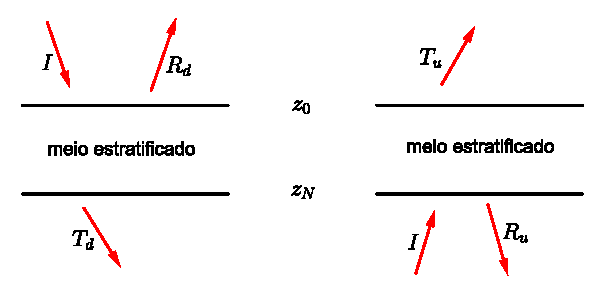
\includegraphics[scale=1.6]{ondas_ascen_descen}
\caption{\textit{Dire\c{c}\~ao e sentido de propaga\c{c}\~ao de ondas ascendentes e descendentes em camadas homog\^eneas.}}
\label{fig.ondas_ascen_descen}
\end{figure}
Vamos usar a const\^ancia da fun\c{c}\~ao dada na equa\c{c}\~ao \ref{eq.G(V,W)} para igualar seus valores calculados no topo e no fundo da pilha de camadas. Mas aqui, vamos tomar as ondas $V$ e $W$ com for\c{c}a $I$ em sentido descendente e ascendente, respectivamente.  
\begin{equation}
\begin{bmatrix}
R_d^\top&I
\end{bmatrix}
\begin{bmatrix}
0&I\\
-I&0
\end{bmatrix}
\begin{bmatrix}
T_u\\
0
\end{bmatrix}
=
\begin{bmatrix}
0&T_d^\top
\end{bmatrix}
\begin{bmatrix}
0&I\\
-I&0
\end{bmatrix}
\begin{bmatrix}
I\\
R_u
\end{bmatrix}\,,
\end{equation}
de onde conclu\'imos que
\begin{equation}\label{eq.T}
T_u=T_d^\top\,.
\end{equation}
Podemos ainda calcular o valor da fun\c{c}ao usando somente ondas descendentes $G(V,V)$. Igualando seus valores para o topo e a base da pilha de camadas, temos
\begin{equation}
\begin{bmatrix}
R_d^\top&I
\end{bmatrix}
\begin{bmatrix}
0&I\\
-I&0
\end{bmatrix}
\begin{bmatrix}
R_d\\
0
\end{bmatrix}
=
\begin{bmatrix}
0&R_d^\top
\end{bmatrix}
\begin{bmatrix}
0&I\\
-I&0
\end{bmatrix}
\begin{bmatrix}
I\\
R_d
\end{bmatrix}\,,
\end{equation}
de onde conclu\'imos que 
\begin{equation}\label{eq.R_d}
R_d=R_d^\top\,.
\end{equation}
Analogamente, para ondas ascendentes $G(W,W)$, temos \begin{equation}\label{eq.R_u}
R_u=R_u^\top\,.
\end{equation}
Utilizando as equa\c{c}\~oes \ref{eq.T}, \ref{eq.R_d} e \ref{eq.R_u}, podemos definir uma matriz $R$ onde as componentes representam todas as ondas refletidas e transmitidas,
\begin{equation}
R=
\begin{bmatrix}
R_d&T_u\\
T_d&R_u
\end{bmatrix}\,,
\end{equation}
e verificar que 
\begin{equation}
R=R^\top\,.
\end{equation}
A matriz $R$ est\'a relacionada \`a matriz $S$ usada em \textit{Teoria de Dispers\~ao} de ondas,
\begin{equation}
S=
\begin{bmatrix}
T_d&R_u\\
R_d&T_u
\end{bmatrix}\,.
\end{equation}
\chapter{Solu\c{c}\~ao das Equa\c{c}\~oes \ref{eq.matricial_1}-\ref{eq.matricial_4} na Aus\^encia de Fonte}\label{sec.ausencia_fonte}

Vamos determinar inicialmente a solu\c{c}\~ao das equa\c{c}\~oes \ref{eq.matricial_1}-\ref{eq.matricial_4} considerando o meio homog\^eneo e livre de fonte de onda sismica. Apos a diagonalizacao dessas equacoes, podemos aplicar um m\'etodo utilizado por alguns autores como \cite{Ursin-1983}, \cite{Azeredo_2013}, \cite{White_Zhou_2006}, \cite{miranda_2016} entre outros, para determinar as solu\c{c}\~oes na aus\^encia de fonte. Esse mesmo metodo pode ser utilizado para determinar as solucoes na presenca de fonte como veremos no capitulo \ref{sec.presenca_fonte}. Aus\^encia de fonte significa que temos $\mathbf{S}^{(m)}=0$ para $m=1,2,3,4\,$ na equa\c{c}\~ao \ref{eq.matricial}. A matriz $\mathbf{M}^{(m)}$ \'e constante onde as submatrizes na diagonal principal s\~ao nulas e as submatrizes na diagonal secund\'aria s\~ao sim\'etricas. 



\section{Ondas Ascendentes e Ondas Descendentes}

Vamos redefinir o vetor de ondas como
\begin{equation}\label{eq.Phi}
\mathbf{\Phi}=L\,\mathbf{\Psi}.
\end{equation}
Substituindo a equa\c{c}\~ao \ref{eq.Phi} na equa\c{c}\~ao \ref{eq.matricial}, temos
\begin{equation}\label{eq.matricial_sem_fonte}
\frac{\partial\,\mathbf{\Psi}}{\partial\,z} =-\,i\,\omega\,L^{-1}M\,L\,\mathbf{\Psi},
\end{equation}
onde o sobrescrito $m$ est\'a sendo omitido por quest\~ao de simplicidade.
De acordo com a subse\c{c}\~ao \ref{sec.diagonalizacao_ursin}, temos que as matrizes $M$ e $\tilde{\Lambda}$ s\~ao semelhantes, assim
\begin{equation*}
\tilde{\Lambda}=L^{-1}M\,L.
\end{equation*}
Substituindo $\tilde{\Lambda}$ na equa\c{c}\~ao \ref{eq.matricial_sem_fonte}, temos
\begin{equation}\label{eq.matricial_sem_fonte_2}
\frac{\partial\,\mathbf{\Psi}}{\partial\,z} =-\,i\,\omega\,\tilde{\Lambda}\,\mathbf{\Psi}.
\end{equation}
Ainda de acordo com a subse\c{c}\~ao \ref{sec.diagonalizacao_ursin}, podemos escrever
\begin{equation}
\tilde{\Lambda}=
\begin{pmatrix}
\Lambda&0\\
0&-\Lambda
\end{pmatrix},
\end{equation}
onde $\Lambda$ \'e uma submatriz diagonal contendo os autovalores $q_i$.
Definindo
\begin{equation}\label{eq.definicao_psi}
\mathbf{\Psi}=
\begin{pmatrix}
\mathbf{U}\\
\mathbf{D}
\end{pmatrix}
\end{equation}
e usando o fato de que $\tilde{\Lambda}$ \'e uma matriz diagonal, podemos resolver a equa\c{c}\~ao diferencial \ref{eq.matricial_sem_fonte_2} e expressar a solu\c{c}\~ao na forma
\begin{align}\nonumber
\mathbf{\Psi}(z)&=e^{-i\,\omega\,\tilde{\Lambda}(z-z_0)}\mathbf{\Psi}(z_0)\\\label{eq.solucao_psi}
&=\begin{pmatrix}
e^{-i\,\omega\,\Lambda(z-z_0)}\,\mathbf{U}(z_0)\\
e^{i\,\omega\,\Lambda(z-z_0)}\,\,\,\mathbf{D}(z_0)
\end{pmatrix}.
\end{align}
Desta maneira, $\mathbf{U}$ representa ondas ascendentes e $\mathbf{D}$ representa ondas descendentes, $z_0$ \'e um ponto fixo na mesma regi\~ao livre de fonte de $z$ e $e^{\pm i\,\omega\,\Lambda(z-z_0)}$ \'e uma matriz diagonal onde o $i$-ésimo elemento da diagonal principal \'e dado por $e^{\pm i\,\omega\,q_i(z-z_0)}$. 

\section{Matriz de Salto para Camadas Estratificadas}

A profundidade onde encontra-se uma interface entre duas camadas estratificadas ser\'a denotada por $\overline{z}$, onde as quantidades avaliadas exatamente abaixo da interface ser\'a denotada por $\overline{z}^+$ e as quantidades avaliadas exatamente acima da interface ser\'a denotada por $\overline{z}^-$.
De acordo com TAL, temos a continuidade de $\mathbf{\Phi}$ atrav\'es das fronteiras entre as camadas, assim \'e v\'alida a rela\c{c}\~ao $\mathbf{\Phi}^+=\mathbf{\Phi}^-$. Substituindo a equa\c{c}\~ao \ref{eq.Phi}, temos 
\begin{align}\nonumber
L^+\mathbf{\Psi}^+&=L^-\mathbf{\Psi}^-\\\nonumber
\mathbf{\Psi}^+&=(L^+)^{-1}L^-\mathbf{\Psi}^-\\\label{eq.psi_matriz_salto}
\mathbf{\Psi}^+&=J\,\mathbf{\Psi}^-,
\end{align}
onde $J=(L^+)^{-1}L^-$ \'e denominada \textit{matriz de salto}. Pela subse\c{c}\~ao \ref{sec.diagonalizacao_ursin} podemos verificar que
\begin{equation}\label{eq.matriz_L}
L=\frac{1}{\sqrt{2}}
\begin{pmatrix}
L_1&L_1\\
L_2&-L_2
\end{pmatrix},
\end{equation}
e podemos expressar a matriz de salto como
\begin{equation}
J=
\begin{pmatrix}
J_A&J_B\\
J_B&J_A
\end{pmatrix},
\end{equation}
onde $J_A$ e $J_B$ s\~ao dadas por
\begin{align}\label{eq.j_a}
J_A&=\frac{1}{2}\left[(L_2^+)^\top L_1^-+(L_1^+)^\top L_2^-\right]\\\label{eq.j_b}
J_B&=\frac{1}{2}\left[(L_2^+)^\top L_1^--(L_1^+)^\top L_2^-\right].
\end{align}
Com uma simples multiplica\c{c}\~ao de matrizes temos que
\begin{align}\nonumber
J^{-1}&=(L^-)^{-1}L^+\\\label{eq.inversa_matriz_salto}
&=
\begin{pmatrix}
J_A^\top&-J_B^\top\\
-J_B^\top&J_A^\top
\end{pmatrix}.
\end{align}

\section{Matriz de Reflex\~ao e Matriz de Transmiss\~ao}

Considere um meio estratificado, homog\^eneo no interior de cada camada, com $N$ interfaces nas profundidades $0<z_1<z_2<...<z_N<\infty$ e sem exist\^encia de fonte nessas camadas. 

\subsection{Reflex\~ao e Transmiss\~ao na \'Ultima Interface}
Pela figura \ref{fig.ondas_em_zn}, considerando que n\~ao h\'a ondas ascendentes depois da \'ultima interface em $z=z_N$, podemos substituir a defini\c{c}\~ao \ref{eq.definicao_psi} na equa\c{c}\~ao \ref{eq.psi_matriz_salto} e obter
\begin{align*}
\mathbf{\Psi}_N^-&=J_N^{-1}\,\mathbf{\Psi}_N^+\\\\
\begin{pmatrix}
\mathbf{U}_N^-\\
\mathbf{D}_N^-
\end{pmatrix}
&=J_N^{-1}\,
\begin{pmatrix}
0\\
\mathbf{D}_N^+
\end{pmatrix}.
\end{align*}

\begin{figure}
\centering
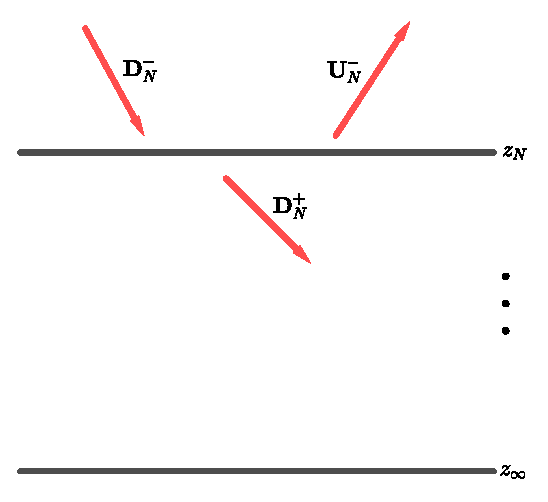
\includegraphics[scale=1]{ondas_em_zn}
\caption{\textit{Ondas ascendentes e descendentes na \'ultima interface.}}
\label{fig.ondas_em_zn}
\end{figure}

Substituindo a equa\c{c}\~ao \ref{eq.inversa_matriz_salto} na equa\c{c}\~ao anterior, temos
\begin{align*}
\begin{pmatrix}
\mathbf{U}_N^-\\
\mathbf{D}_N^-
\end{pmatrix}
&=
\begin{pmatrix}
J_{A,N}^\top&-J_{B,N}^\top\\
-J_{B,N}^\top&J_{A,N}^\top
\end{pmatrix}
\,
\begin{pmatrix}
0\\
\mathbf{D}_N^+
\end{pmatrix}\\\\
&=
\begin{pmatrix}
-J_{B,N}^\top \mathbf{D}_N^+\\
 J_{A,N}^\top \mathbf{D}_N^+
\end{pmatrix},
\end{align*}
ou seja,
\begin{align*}
\mathbf{U}_N^-&=-J_{B,N}^\top J_{A,N}^{-\top}\mathbf{D}_N^-\\
\mathbf{D}_N^+&=J_{A,N}^{-\top}\mathbf{D}_N^-.
\end{align*}
Assim, vemos que para computar uma onda refletida, ou seja, uma onda ascendente a partir de uma interface entre camadas, usamos uma \textit{matriz de reflex\~ao} que fica definida como
\begin{equation}\label{eq.reflexao_N}
\Gamma_N=-J_{B,N}^\top J_{A,N}^{-\top}.
\end{equation} 
Analogamente, vemos que para computar uma onda transmitida, ou seja, uma onda descendente a partir de uma interface entre camadas, usamos uma \textit{matriz de transmiss\~ao} que fica definida como
\begin{equation}\label{eq.transmissao_N}
T_N=J_{A,N}^{-\top}.
\end{equation} 

\subsection{Reflex\~ao e Transmiss\~ao numa Interface Qualquer}
Definimos a espessura de uma camada, a partir da interface superior, como
\begin{equation}
\Delta\,z_m=z_{m+1}-z_m,\qquad m=1,2,...,N-1,
\end{equation}
e temos que uma onda se propagando da interface na profundidade $z_m$ at\'e a interface em $z_{m+1}$ percorre uma profundidade total $\Delta\,z_m$. O valor dessa onda no fim da trajet\'oria, quando $z=z_{m+1}$, \'e aproximadamente igual a $\mathbf{\Psi}^-_{m+1}$, conforme a figura \ref{fig.N_interfaces}. Assim, usando a solu\c{c}\~ao \ref{eq.solucao_psi} podemos escrever
\begin{equation}\label{eq.solucao_delta_zm}
\mathbf{\Psi}^-_{m+1}=e^{-i\,\omega\tilde{\Lambda}_m\Delta\,z_m}\mathbf{\Psi}^+_m.
\end{equation}

\begin{figure}
\centering
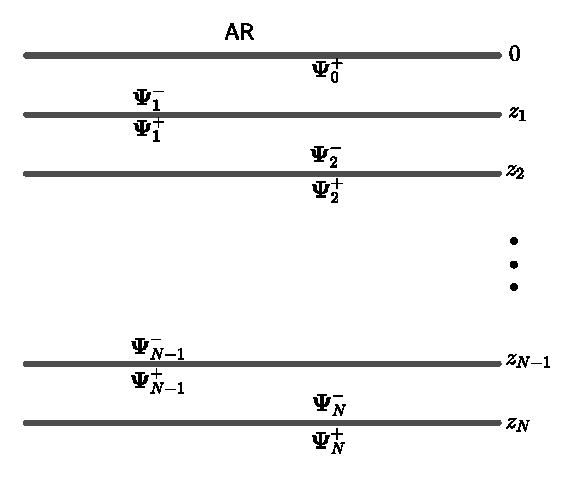
\includegraphics[scale=1]{n_interfaces}
\caption{\textit{Visualizacao de $N$ interfaces em subsuperficie e a notacao das ondas nas proximadades de cada interface.}}
\label{fig.N_interfaces}
\end{figure}

Sabendo que essa onda se propagando na camada abaixo da interface em $z_m$ veio da camada anterior, podemos usar a matriz de salto na equa\c{c}\~ao \ref{eq.psi_matriz_salto} e escrever
\begin{align}\label{eq.salto_m}
\mathbf{\Psi}^+_{m}&=J_m\,\mathbf{\Psi}^-_m.\\
\end{align}
Substituindo a equa\c{c}\~ao \ref{eq.salto_m} na equa\c{c}\~ao \ref{eq.solucao_delta_zm}, temos
\begin{align*}
\mathbf{\Psi}^-_{m+1}&=e^{-i\,\omega\tilde{\Lambda}_m\Delta\,z_m}\mathbf{\Psi}^+_m\\
\mathbf{\Psi}^-_{m+1}&=e^{-i\,\omega\tilde{\Lambda}_m\Delta\,z_m}J_m\,\mathbf{\Psi}^-_m\\
\mathbf{\Psi}^-_m&=J^{-1}_me^{i\,\omega\tilde{\Lambda}_m\Delta\,z_m}\mathbf{\Psi}^-_{m+1}
\end{align*}
Substituindo a equa\c{c}\~ao \ref{eq.definicao_psi} e a equa\c{c}\~ao \ref{eq.inversa_matriz_salto}, temos
\begin{align}\label{eq.refle_trans_1}
\mathbf{U}_m^-&=J^\top_{A,m}e^{i\,\omega\Lambda_m\Delta\,z_m}\mathbf{U}^-_{m+1}-J^\top_{B,m}e^{-i\,\omega\Lambda_m\Delta\,z_m}\mathbf{D}^-_{m+1}\\\nonumber\\\label{eq.refle_trans_2}
\mathbf{D}_m^-&=-J^\top_{B,m}e^{i\,\omega\Lambda_m\Delta\,z_m}\mathbf{U}^-_{m+1}+J^\top_{A,m}e^{-i\,\omega\Lambda_m\Delta\,z_m}\mathbf{D}^-_{m+1}.
\end{align}
Assim como definimos matriz de reflex\~ao para a \'ultima interface em $z_N$, podemos definir a matriz de reflex\~ao para uma interface qualquer, ou seja,
\begin{equation}\label{eq.reflexao_m+1}
\mathbf{U}^-_{m+1}=\Gamma_{m+1}\mathbf{D}^-_{m+1}.
\end{equation}
Substituindo a equa\c{c}\~ao \ref{eq.reflexao_m+1} na equa\c{c}\~ao \ref{eq.refle_trans_1} e na equa\c{c}\~ao \ref{eq.refle_trans_2}, temos
\begin{align}\label{eq.refle_trans_3}
\mathbf{U}_m^-&=(J^\top_{A,m}e^{i\,\omega\Lambda_m\Delta\,z_m}\Gamma_{m+1}-J^\top_{B,m}e^{-i\,\omega\Lambda_m\Delta\,z_m})\mathbf{D}^-_{m+1}\\\nonumber\\\label{eq.refle_trans_4}
\mathbf{D}_m^-&=(-J^\top_{B,m}e^{i\,\omega\Lambda_m\Delta\,z_m}\Gamma_{m+1}+J^\top_{A,m}e^{-i\,\omega\Lambda_m\Delta\,z_m})\mathbf{D}^-_{m+1}\,.
\end{align}
Substituindo a equa\c{c}\~ao \ref{eq.refle_trans_4} na equa\c{c}\~ao \ref{eq.refle_trans_3}, temos
\begin{align*}
\mathbf{U}_m^-&=(J^\top_{A,m}e^{i\,\omega\Lambda_m\Delta\,z_m}\Gamma_{m+1}-J^\top_{B,m}e^{-i\,\omega\Lambda_m\Delta\,z_m})\\
&\,\,\cdot\,\,(-J^\top_{B,m}e^{i\,\omega\Lambda_m\Delta\,z_m}\Gamma_{m+1}+J^\top_{A,m}e^{-i\,\omega\Lambda_m\Delta\,z_m})^{-1}\mathbf{D}_m^-\,,
\end{align*}
de onde podemos concluir que a matriz de reflex\~ao em uma interface em $z_m$ qualquer \'e dada por
\begin{align*}
\Gamma_{m}&=(J^\top_{A,m}e^{i\,\omega\Lambda_m\Delta\,z_m}\Gamma_{m+1}-J^\top_{B,m}e^{-i\,\omega\Lambda_m\Delta\,z_m})\\
&\,\,\cdot\,\,(-J^\top_{B,m}e^{i\,\omega\Lambda_m\Delta\,z_m}\Gamma_{m+1}+J^\top_{A,m}e^{-i\,\omega\Lambda_m\Delta\,z_m})^{-1},
\end{align*}
ou
\begin{align}\nonumber
\Gamma_{m}&=(J^\top_{A,m}e^{i\,\omega\Lambda_m\Delta\,z_m}\Gamma_{m+1}e^{i\,\omega\Lambda_m\Delta\,z_m}-J^\top_{B,m})\\\label{eq.matriz_reflexao_m}
&\,\,\cdot\,\,(-J^\top_{B,m}e^{i\,\omega\Lambda_m\Delta\,z_m}\Gamma_{m+1}e^{i\,\omega\Lambda_m\Delta\,z_m}+J^\top_{A,m})^{-1}.
\end{align}
Quando uma onda atinge uma interface, alem da possibilidade de reflexao ha tambem a possibilidade de trasmissao da onda para a camada inferior. De maneira analoga ao desenvolvido para reflexao de ondas, podemos deduzir a matriz para a transmissao de ondas em uma interface qualquer, que eh dada por
\begin{equation}\label{eq.matriz_transmissao_m}
T_m=T_{m+1}e^{i\,\omega\,\Lambda\Delta\,z_m}(-J^\top_{B,m}e^{i\,\omega\Lambda_m\Delta\,z_m}\Gamma_{m+1}e^{i\,\omega\Lambda_m\Delta\,z_m}+J^\top_{A,m})^{-1}.
\end{equation}
A validade das equacoes \ref{eq.matriz_reflexao_m} e \ref{eq.matriz_transmissao_m} para qualquer interface pode ser demonstrada por inducao sobre $m$, e todas as matrizes de reflexao e transmissao podem ser computadas por recurssao partindo das equacoes \ref{eq.reflexao_N} e \ref{eq.transmissao_N}.







\bibliographystyle{plainnat}
\bibliography{referencias}

\end{document}